%  A simple AAU report template.
%  2015-05-08 v. 1.2.0
%  Copyright 2010-2015 by Jesper Kjær Nielsen <jkn@es.aau.dk>
%
%  This is free software: you can redistribute it and/or modify
%  it under the terms of the GNU General Public License as published by
%  the Free Software Foundation, either version 3 of the License, or
%  (at your option) any later version.
%
%  This is distributed in the hope that it will be useful,
%  but WITHOUT ANY WARRANTY; without even the implied warranty of
%  MERCHANTABILITY or FITNESS FOR A PARTICULAR PURPOSE.  See the
%  GNU General Public License for more details.
%
%  You can find the GNU General Public License at <http://www.gnu.org/licenses/>.
%
%  A simple AAU report template.
%  2015-05-08 v. 1.2.0
%  Copyright 2010-2015 by Jesper Kjær Nielsen <jkn@es.aau.dk>
%
%  This is free software: you can redistribute it and/or modify
%  it under the terms of the GNU General Public License as published by
%  the Free Software Foundation, either version 3 of the License, or
%  (at your option) any later version.
%
%  This is distributed in the hope that it will be useful,
%  but WITHOUT ANY WARRANTY; without even the implied warranty of
%  MERCHANTABILITY or FITNESS FOR A PARTICULAR PURPOSE.  See the
%  GNU General Public License for more details.
%
%  You can find the GNU General Public License at <http://www.gnu.org/licenses/>.
%
\documentclass[11pt,twoside,a4paper,openright]{report}
%%%%%%%%%%%%%%%%%%%%%%%%%%%%%%%%%%%%%%%%%%%%%%%%
% Language, Encoding and Fonts
% http://en.wikibooks.org/wiki/LaTeX/Internationalization
%%%%%%%%%%%%%%%%%%%%%%%%%%%%%%%%%%%%%%%%%%%%%%%%
% Select encoding of your inputs. Depends on
% your operating system and its default input
% encoding. Typically, you should use
%   Linux  : utf8 (most modern Linux distributions)
%            latin1 
%   Windows: ansinew
%            latin1 (works in most cases)
%   Mac    : applemac
% Notice that you can manually change the input
% encoding of your files by selecting "save as"
% an select the desired input encoding. 
\usepackage[utf8]{inputenc}
% Make latex understand and use the typographic
% rules of the language used in the document.
\usepackage[danish,english]{babel}
% Use the palatino font
\usepackage[sc]{mathpazo}
\linespread{1.05}         % Palatino needs more leading (space between lines)
% Choose the font encoding
\usepackage[T1]{fontenc}
%%%%%%%%%%%%%%%%%%%%%%%%%%%%%%%%%%%%%%%%%%%%%%%%
% Graphics and Tables
% http://en.wikibooks.org/wiki/LaTeX/Importing_Graphics
% http://en.wikibooks.org/wiki/LaTeX/Tables
% http://en.wikibooks.org/wiki/LaTeX/Colors
%%%%%%%%%%%%%%%%%%%%%%%%%%%%%%%%%%%%%%%%%%%%%%%%
% load a colour package
\usepackage{xcolor}
\definecolor{aaublue}{RGB}{33,26,82}% dark blue
% The standard graphics inclusion package
\usepackage{graphicx}
% Set up how figure and table captions are displayed
\usepackage{caption}
\captionsetup{%
  font=footnotesize,% set font size to footnotesize
  labelfont=bf % bold label (e.g., Figure 3.2) font
}
% Make the standard latex tables look so much better
\usepackage{array,booktabs}
% Enable the use of frames around, e.g., theorems
% The framed package is used in the example environment
\usepackage{framed}

%%%%%%%%%%%%%%%%%%%%%%%%%%%%%%%%%%%%%%%%%%%%%%%%
% Mathematics
% http://en.wikibooks.org/wiki/LaTeX/Mathematics
%%%%%%%%%%%%%%%%%%%%%%%%%%%%%%%%%%%%%%%%%%%%%%%%
% Defines new environments such as equation,
% align and split 
\usepackage{amsmath}
% Adds new math symbols
\usepackage{amssymb}
% Use theorems in your document
% The ntheorem package is also used for the example environment
% When using thmmarks, amsmath must be an option as well. Otherwise \eqref doesn't work anymore.
\usepackage[framed,amsmath,thmmarks]{ntheorem}

%%%%%%%%%%%%%%%%%%%%%%%%%%%%%%%%%%%%%%%%%%%%%%%%
% Page Layout
% http://en.wikibooks.org/wiki/LaTeX/Page_Layout
%%%%%%%%%%%%%%%%%%%%%%%%%%%%%%%%%%%%%%%%%%%%%%%%
% Change margins, papersize, etc of the document
\usepackage[
  inner=28mm,% left margin on an odd page
  outer=41mm,% right margin on an odd page
  ]{geometry}
% Modify how \chapter, \section, etc. look
% The titlesec package is very configureable
\usepackage{titlesec}
\titleformat{\chapter}[display]{\normalfont\huge\bfseries}{\chaptertitlename\ \thechapter}{20pt}{\Huge}
\titleformat*{\section}{\normalfont\Large\bfseries}
\titleformat*{\subsection}{\normalfont\large\bfseries}
\titleformat*{\subsubsection}{\normalfont\normalsize\bfseries}
%\titleformat*{\paragraph}{\normalfont\normalsize\bfseries}
%\titleformat*{\subparagraph}{\normalfont\normalsize\bfseries}

% Clear empty pages between chapters
\let\origdoublepage\cleardoublepage
\newcommand{\clearemptydoublepage}{%
  \clearpage
  {\pagestyle{empty}\origdoublepage}%
}
\let\cleardoublepage\clearemptydoublepage

% Change the headers and footers
\usepackage{fancyhdr}
\pagestyle{fancy}
\fancyhf{} %delete everything
\renewcommand{\headrulewidth}{0pt} %remove the horizontal line in the header
\fancyhead[RE]{\small\nouppercase\leftmark} %even page - chapter title
\fancyhead[LO]{\small\nouppercase\rightmark} %uneven page - section title
\fancyhead[LE,RO]{\thepage} %page number on all pages
% Do not stretch the content of a page. Instead,
% insert white space at the bottom of the page
\raggedbottom
% Enable arithmetics with length. Useful when
% typesetting the layout.
\usepackage{calc}

%%%%%%%%%%%%%%%%%%%%%%%%%%%%%%%%%%%%%%%%%%%%%%%%
% Bibliography
% http://en.wikibooks.org/wiki/LaTeX/Bibliography_Management
%%%%%%%%%%%%%%%%%%%%%%%%%%%%%%%%%%%%%%%%%%%%%%%%
\usepackage[backend=bibtex,
  bibencoding=utf8
  ]{biblatex}
\addbibresource{bib/mybib}

%%%%%%%%%%%%%%%%%%%%%%%%%%%%%%%%%%%%%%%%%%%%%%%%
% Misc
%%%%%%%%%%%%%%%%%%%%%%%%%%%%%%%%%%%%%%%%%%%%%%%%
% Add bibliography and index to the table of
% contents
\usepackage[nottoc]{tocbibind}
% Add the command \pageref{LastPage} which refers to the
% page number of the last page
\usepackage{lastpage}
% Add todo notes in the margin of the document
\usepackage[
%  disable, %turn off todonotes
  colorinlistoftodos, %enable a coloured square in the list of todos
  textwidth=\marginparwidth, %set the width of the todonotes
  textsize=scriptsize, %size of the text in the todonotes
  ]{todonotes}

%%%%%%%%%%%%%%%%%%%%%%%%%%%%%%%%%%%%%%%%%%%%%%%%
% Hyperlinks
% http://en.wikibooks.org/wiki/LaTeX/Hyperlinks
%%%%%%%%%%%%%%%%%%%%%%%%%%%%%%%%%%%%%%%%%%%%%%%%
% Enable hyperlinks and insert info into the pdf
% file. Hypperref should be loaded as one of the 
% last packages
\usepackage{hyperref}
\hypersetup{%
	pdfpagelabels=true,%
	plainpages=false,%
	pdfauthor={Author(s)},%
	pdftitle={Title},%
	pdfsubject={Subject},%
	bookmarksnumbered=true,%
	colorlinks=false,%
	citecolor=black,%
	filecolor=black,%
	linkcolor=black,% you should probably change this to black before printing
	urlcolor=black,%
	pdfstartview=FitH%
}% package inclusion and set up of the document
% see, e.g., http://en.wikibooks.org/wiki/LaTeX/Formatting#Hyphenation
% for more information on word hyphenation
\hyphenation{ex-am-ple hy-phen-a-tion short}
\hyphenation{long la-tex}% 
%  A simple AAU report template.
%  2015-05-08 v. 1.2.0
%  Copyright 2010-2015 by Jesper Kjær Nielsen <jkn@es.aau.dk>
%
%  This is free software: you can redistribute it and/or modify
%  it under the terms of the GNU General Public License as published by
%  the Free Software Foundation, either version 3 of the License, or
%  (at your option) any later version.
%
%  This is distributed in the hope that it will be useful,
%  but WITHOUT ANY WARRANTY; without even the implied warranty of
%  MERCHANTABILITY or FITNESS FOR A PARTICULAR PURPOSE.  See the
%  GNU General Public License for more details.
%
%  You can find the GNU General Public License at <http://www.gnu.org/licenses/>.
%
%
%
% see, e.g., http://en.wikibooks.org/wiki/LaTeX/Customizing_LaTeX#New_commands
% for more information on how to create macros

%%%%%%%%%%%%%%%%%%%%%%%%%%%%%%%%%%%%%%%%%%%%%%%%
% Macros for the titlepage
%%%%%%%%%%%%%%%%%%%%%%%%%%%%%%%%%%%%%%%%%%%%%%%%
%Creates the aau titlepage
\newcommand{\aautitlepage}[3]{%
  {
    %set up various length
    \ifx\titlepageleftcolumnwidth\undefined
      \newlength{\titlepageleftcolumnwidth}
      \newlength{\titlepagerightcolumnwidth}
    \fi
    \setlength{\titlepageleftcolumnwidth}{0.5\textwidth-\tabcolsep}
    \setlength{\titlepagerightcolumnwidth}{\textwidth-2\tabcolsep-\titlepageleftcolumnwidth}
    %create title page
    \thispagestyle{empty}
    \noindent%
    \begin{tabular}{@{}ll@{}}
      \parbox{\titlepageleftcolumnwidth}{
        \iflanguage{danish}{%
          
\includegraphics[width=\titlepageleftcolumnwidth]{figures/aau_logo_da}
        }{%
          
\includegraphics[width=\titlepageleftcolumnwidth]{figures/aau_logo_en}
        }
      } &
      \parbox{\titlepagerightcolumnwidth}{\raggedleft\sf\small
        #2
      }\bigskip\\
       #1 &
      \parbox[t]{\titlepagerightcolumnwidth}{%
      \textbf{Abstract:}\bigskip\par
        \fbox{\parbox{\titlepagerightcolumnwidth-2\fboxsep-2\fboxrule}{%
          #3
        }}
      }\\
    \end{tabular}
    \vfill
    \iflanguage{danish}{%
      \noindent{\footnotesize\emph{Rapportens indhold er frit tilgængeligt, men offentliggørelse (med kildeangivelse) må kun ske efter aftale med forfatterne.}}
    }{%
      \noindent{\footnotesize\emph{The content of this report is freely available, but publication (with reference) may only be pursued due to agreement with the author.}}
    }
    \clearpage
  }
}

%Create english project info
\newcommand{\englishprojectinfo}[8]{%
  \parbox[t]{\titlepageleftcolumnwidth}{
    \textbf{Title:}\\ #1\bigskip\par
    \textbf{Theme:}\\ #2\bigskip\par
    \textbf{Project Period:}\\ #3\bigskip\par
    \textbf{Project Group:}\\ #4\bigskip\par
    \textbf{Participant(s):}\\ #5\bigskip\par
    \textbf{Supervisor(s):}\\ #6\bigskip\par
    \textbf{Copies:} #7\bigskip\par
    \textbf{Page Numbers:} \pageref{LastPage}\bigskip\par
    \textbf{Date of Completion:}\\ #8
  }
}

%Create danish project info
\newcommand{\danishprojectinfo}[8]{%
  \parbox[t]{\titlepageleftcolumnwidth}{
    \textbf{Titel:}\\ #1\bigskip\par
    \textbf{Tema:}\\ #2\bigskip\par
    \textbf{Projektperiode:}\\ #3\bigskip\par
    \textbf{Projektgruppe:}\\ #4\bigskip\par
    \textbf{Deltager(e):}\\ #5\bigskip\par
    \textbf{Vejleder(e):}\\ #6\bigskip\par
    \textbf{Oplagstal:} #7\bigskip\par
    \textbf{Sidetal:} \pageref{LastPage}\bigskip\par
    \textbf{Afleveringsdato:}\\ #8
  }
}

%%%%%%%%%%%%%%%%%%%%%%%%%%%%%%%%%%%%%%%%%%%%%%%%
% An example environment
%%%%%%%%%%%%%%%%%%%%%%%%%%%%%%%%%%%%%%%%%%%%%%%%
\theoremheaderfont{\normalfont\bfseries}
\theorembodyfont{\normalfont}
\theoremstyle{break}
\def\theoremframecommand{{\color{gray!50}\vrule width 5pt \hspace{5pt}}}
\newshadedtheorem{exa}{Example}[chapter]
\newenvironment{example}[1]{%
		\begin{exa}[#1]
}{%
		\end{exa}
}% my new macros

\begin{document}
%frontmatter
\pagestyle{empty} %disable headers and footers
\pagenumbering{roman} %use roman page numbering in the frontmatter
%  A simple AAU report template.
%  2015-05-08 v. 1.2.0
%  Copyright 2010-2015 by Jesper Kjær Nielsen <jkn@es.aau.dk>
%
%  This is free software: you can redistribute it and/or modify
%  it under the terms of the GNU General Public License as published by
%  the Free Software Foundation, either version 3 of the License, or
%  (at your option) any later version.
%
%  This is distributed in the hope that it will be useful,
%  but WITHOUT ANY WARRANTY; without even the implied warranty of
%  MERCHANTABILITY or FITNESS FOR A PARTICULAR PURPOSE.  See the
%  GNU General Public License for more details.
%
%  You can find the GNU General Public License at <http://www.gnu.org/licenses/>.
%
\pdfbookmark[0]{Front page}{label:frontpage}%
\begin{titlepage}
  \addtolength{\hoffset}{0.5\evensidemargin-0.5\oddsidemargin} %set equal margins on the frontpage - remove this line if you want default margins
  \noindent%
  \begin{tabular}{@{}p{\textwidth}@{}}
    \toprule[2pt]
    \midrule
    \vspace{0.2cm}
    \begin{center}
    \Huge{\textbf{
      Survey On Application Software% insert your title here
    }}
    \end{center}
    \begin{center}
      \Large{- Industrial Insights -% insert your subtitle here
      }
    \end{center}
    \vspace{0.2cm}\\
    \midrule
    \toprule[2pt]
  \end{tabular}
  \vspace{4 cm}
  \begin{center}
    {\large
      Project Report%Insert document type (e.g., Project Report)
    }\\
    \vspace{0.2cm}
    {\Large
      Aarthi Babu%Insert your group name or real names here
    }\\
     \vspace{0.2cm}
    {\Large
      Raja Gunasekaran%Insert your group name or real names here    
    }\\
  \end{center}
  \vfill
  \begin{center}
  University Of Northern British Columbia\\
  Computer Science
  \end{center}
\end{titlepage}
\clearpage
%\thispagestyle{empty}
{\small
\strut\vfill % push the content to the bottom of the page
\noindent Copyright \copyright{} Aalborg University 2015\par
\vspace{0.2cm}
\noindent Here you can write something about which tools and software you have used for typesetting the document, running simulations and creating figures. If you do not know what to write, either leave this page blank or have a look at the colophon in some of your books.
}
\clearpage
%\pdfbookmark[0]{English title page}{label:titlepage_en}
\aautitlepage{%
  \englishprojectinfo{
    Project Title %title
  }{%
    Scientific Theme %theme
  }{%
    Fall Semester 2010 %project period
  }{%
    XXX % project group
  }{%
    %list of group members
    Author 1\\ 
    Author 2\\
    Author 3
  }{%
    %list of supervisors
    Supervisor 1\\
    Supervisor 2
  }{%
    1 % number of printed copies
  }{%
    \today % date of completion
  }%
}{%department and address
  \textbf{Electronics and IT}\\
  Aalborg University\\
  \href{http://www.aau.dk}{http://www.aau.dk}
}{% the abstract
  Here is the abstract
}

\cleardoublepage
{\selectlanguage{danish}
\pdfbookmark[0]{Danish title page}{label:titlepage_da}
\aautitlepage{%
  \danishprojectinfo{
    Rapportens titel %title
  }{%
    Semestertema %theme
  }{%
    Efterårssemestret 2010 %project period
  }{%
    XXX % project group
  }{%
    %list of group members
    Forfatter 1\\ 
    Forfatter 2\\
    Forfatter 3
  }{%
    %list of supervisors
    Vejleder 1\\
    Vejleder 2
  }{%
    1 % number of printed copies
  }{%
    \today % date of completion
  }%
}{%department and address
  \textbf{Elektronik og IT}\\
  Aalborg Universitet\\
  \href{http://www.aau.dk}{http://www.aau.dk}
}{% the abstract
  Her er resuméet
}}
\cleardoublepage
\pdfbookmark[0]{Contents}{label:contents}
\pagestyle{fancy} %enable headers and footers again
\tableofcontents
%\listoftodos\chapter*{Preface\markboth{Preface}{Preface}}\label{ch:preface}
\addcontentsline{toc}{chapter}{Preface}
Here is the preface. You should put your signatures at the end of the preface.

\vspace{\baselineskip}\hfill Aalborg University, \today
\vfill\noindent
\begin{minipage}[b]{0.45\textwidth}
 \centering
 \rule{\textwidth}{0.5pt}\\
  Author 1\\
 {\footnotesize <username1@XX.aau.dk>}
\end{minipage}
\hfill
\begin{minipage}[b]{0.45\textwidth}
 \centering
 \rule{\textwidth}{0.5pt}\\
  Author 2\\
 {\footnotesize <username2@XX.aau.dk>}
\end{minipage}
\vspace{3\baselineskip}
\begin{center}
\begin{minipage}[b]{0.45\textwidth}
 \centering
 \rule{\textwidth}{0.5pt}
  Author 3\\
 {\footnotesize <username3@XX.aau.dk>}
\end{minipage}
\end{center}
%\cleardoublepage
%mainmatter
\pagenumbering{arabic} %use arabic page numbering in the mainmatter
\chapter{Introduction}\label{ch:introduction}
		Application	Software is program or group of program customised to perform group of activities for end user. Generally software are classified as system software and application software.System software consists of low-level programs that is designed to run computer's hardware and application programs like compilers, loaders, linkers and so on. Application software resides above system software like database programs, word processors, spreadsheets. In this survey, we focus on the architecture and process involved in development of different types of application software. 

		Software application architecture is the process of designing a structured solution that focuses on how the components in the applications interact with each other, while optimizing common quality attributes such as performance, security, and manageability.The architecture are structured with consideration of user and the business goals.The selection of data structures and algorithms are design concerns which would overlap with architecture concerns.These scenarios where the both of them overlap are discussed in detailed in later chapters.The architecture must be flexible to handle the changes in software or hardware technologies and requirements that are not known in the early stages of design process as the design of the application will evolve during the development stages.
			
	
\section{Command-Line Application}
			
			Technology has come long way since the first computers were created, back around the start of World War II. The first generation of software application are command line programs which are mostly single command at a time and uses it to accomplish all the application requirements in that particular loop. These programs are shared as binaries(executables) which can be compiled from the source code, specific to the architecture. 

\section{Desktop Application}
			
			In spite of early application which was designed to run from mainframe computers and accessed through terminals devices, the proposal of powerful desktop applications which can be run in the local personal computer dethroned the previous generation application software. The mainframe was replaced with server by the client server model which induced distributed application structure that partitions tasks or workload between the service provider (Server) and the service requester (Client).  
			
\section{Web Application}
			
			Steady enhancements in hardware specifications and broadband speeds led to major improvements in the quality and quantity of WWW content. Websites inflated their features beyond static web pages by becoming more interactive with the increase of multimedia content. As browsers and development platforms evolved, and more and more people began to use the internet and email, more businesses established their presence in the online world. These businesses leveraged the emerging interactive capabilities of the web to introduce applications that were served directly to a web browser, and these web applications became very popular.
			Any Web application is a client server application which consist of a client inform of browser and a web server. The business logic of the application is distributed among the server and client where information is exchanged through a channel and the data is stored in the server end.
					 

\section{Mobile Application}
			
			Nowadays, an ever-growing percentage of portable device like smart phones have doubled the number of users accessing the internet  on their smart phones.The need of mobile applications became pretty obvious. Mobile applications should be designed in such a way that the power consumption and processing power is reduced. Android and iOS being the major players in the industry, they natively support java and ObjectiveC as the native language. 
			
			The mobile applications can be categorised into mobile web application, native application and hybrid application.A native application is developed for a certain mobile device (smart phone, tablet, so on). They’re installed directly onto the device. Users typically acquire these applications through an online store or marketplace such as The App Store or Android Apps on Google Play.It was started working as standalone, and in the recent years, we see a lot of integration with the web which is named as hybrid application.


\begin{figure}[!htb]	
  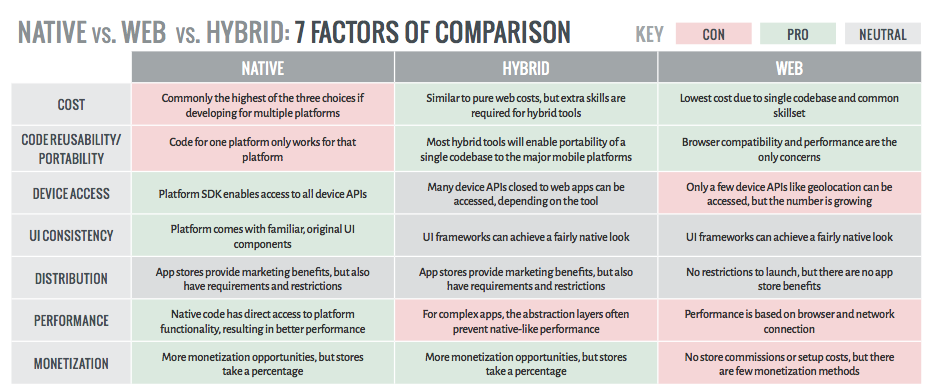
\includegraphics[width=\linewidth,scale = 3]{figures/MobAppTypes.png}
\caption{Native vs Web vs Hybrid}
  \label{fig: Native vs Web vs Hybrid}
\end{figure}	
			
			 Internet-enabled applications that have specific functionality for mobile devices are called as mobile web application. They are accessed through the mobile device’s web browser (i.e. on the iPhone, this is Safari by default) and they don’t need to be downloaded and installed on the device.Although mobile websites and mobile apps aren't the same thing, they generally offer the same features that can help grow business by making it easier for customers to find and reach it. 
			

%\section{Desktop Application}
%You can also have examples in your document such as in example~\ref{ex:simple_example}.
%\begin{example}{An Example of an Example}
%  \label{ex:simple_example}
%  Here is an example with some math
%  \begin{equation}
%    0 = \exp(i\pi)+1\ .
%  \end{equation}
%  You can adjust the colour and the line width in the {\tt macros.tex} file.
%\end{example}
%
%\section{Web Application}
%Well, like this
%\subsection{This is a Subsection}
%and this
%\subsubsection{This is a Subsubsection}
%and this.
%
%\paragraph{A Paragraph}
%You can also use paragraph titles which look like this.
%
%\subparagraph{A Subparagraph} Moreover, you can also use subparagraph titles which look like this\todo{Is it possible to add a subsubparagraph?}. They have a small indentation as opposed to the paragraph titles.
%
%\todo[inline,color=green]{I think that a summary of this exciting chapter should be added.}
%
%\section{Mobile Application}
%Well, like this
%\subsection{This is a Subsection}
%and this
%\subsubsection{This is a Subsubsection}
%and this.
%
%\paragraph{A Paragraph}
%You can also use paragraph titles which look like this.
%
%\subparagraph{A Subparagraph} Moreover, you can also use subparagraph titles which look like this\todo{Is it possible to add a subsubparagraph?}. They have a small indentation as opposed to the paragraph titles.
%
%\todo[inline,color=green]{I think that a summary of this exciting chapter should be added.}
\cleardoublepage
\chapter{Chapter 2 name}\label{ch:ch2label}
Here is chapter 2. If you want to leearn \todo{I think this word is mispelled} more about \LaTeXe{}, have a look at \cite{Madsen2010}, \cite{Oetiker2010} and \cite{Mittelbach2005}.
\missingfigure{We need a figure right here!}
\cleardoublepage
\chapter{Presentation Layer}\label{ch:ch3label}

			The design of presentation layer begins by identifying the potential customer base, and understanding the objectives of the customer and task the user wish to accomplish when using the application. As the main focus of the application design must be user centred, the sequencing of tasks or operations should be designed as per the user expectation. It may be a structured step-by-step user experience or unstructured experience where they can perform more than one tasks simultaneously. One important aspect that has great influence on the choice of technology is functionality required for the user interface. Prioritizing the requirements like rich functionality, user interaction, user responsiveness , user interface , personalization requirements and graphical support will help to choose User Interface Type.
			
			Most of the user interface requirements needs more than one UI type.The frameworks, tool and implementation language used for UI requirements differ according  to the application platform.
			
\section{Mobile Application}
         
            	Mobile application can be classified as thin client and rich client application.Rich client is designed to support the native or hybrid applications which supports offline or intermittent online scenarios. Web or thin clients supports only online  scenarios.Resources constraint should e taken into account while designing user interface for mobile application.
            	
            	Many developers or vendors want to write an application once using single codebase , the run that application in multiple platform with a very small change in codebase. This approach is famously known as Write Once, Run Anywhere (WORA).WORA removes the redundancy in development at the cost of user experience and application performance.This application is called as hybrid mobile application which has native application experience. Improving the performance and user experience are in future roadmap.     
            	
\begin{figure}[!htb]
  \includegraphics[width=\linewidth]{figures/nativeMobApp.png}
	 \caption{Languages - Native Moblie Application }
  \label{fig: Languages - Native Moblie Application}
\end{figure}		            	       	

\subsection{Apache Cordova - Frameworks}
              
              Apache Cordova is an open-source mobile cross-platform development framework which allows you to use standard web technologies - HTML5, CSS3, and JavaScript . In mobile development, this framework extends more than one platform avoiding the implementation time taken for each platform.Applications execute within wrappers targeted to each platform, and rely on standards-compliant API bindings to access each device's capabilities such as sensors, data, network status, etc. It is flexible in developing application which has combination of native application components with a web view that can access device level APIs using Core Plugins.           
            	
\subsection{Ionic - Frameworks}		
              
              Ionic is a free open source framework facilitates the development of hybrid native mobile using web technologies like HTML,Javascript and CSS. Its core is built up with AngularJS javascript framework and supports SASS (Syntactically Awesome Style Sheets) CSS extension . This features qualifies Ionic as a unique framework.It simplifies development and testing of the application by providing client side model view controller architecture. User Interface response is pretty faster than Backbone and Knockout and it possesses a large number of 3rd party plug ins and extensions. Currently Ionic supports iOS and Android devices, Windows phones and FirefoxOS support are considered to be in future roadmap. This framework can be only used for hybrid mobile application.Ionic is built on top of Apache Cordova which is open source mobile development framework.
              

\begin{figure}[!htb]
  \includegraphics[width=\linewidth]{figures/hybridMobApp.png}
	 \caption{Cordova Languages - Hybrid Moblie Application }
  \label{fig: Cordova Languages - Hybrid Moblie Application}
\end{figure}		 

   
\subsection{Mobile Angular UI - Frameworks}     
			
			Mobile Angular UI is an HTML 5 framework which uses bootstrap 3 and AngularJS with better user response. In other words it combines the best of the web framework which enables you to create hybrid application and web application. This framework works well with all browsers including older versions and offers feature of customizing build workflow with GRUNT. Grunt is used run automation  using a task runner with zero effort.
			
\subsection{Xamarin - Frameworks}

				Xamarin applications are written in C\# and compiled to binaries compatible with native device giving access to all the device API through C\# wrappers.To develop application that look like native, Xamarin uses native UI mechanisms for each platform. Recently Xamarin.Forms was released which enables the use of common UI technology, XAML and work on cross platforms using native controls. Xamarin takes advantage of all the third party libraries written for .NET stack 

\begin{figure}[!htb]
  \includegraphics[width=\linewidth]{figures/XamarinhybridApp.png}
	 \caption{ Xamarin Languages - Hybrid Moblie Application }
  \label{fig: Xamarin Languages - Hybrid Moblie Application}
\end{figure}							
			



\section{Web Application}

				Server-side HTML, JS generation widgets (AJAX) and Service-oriented single-page are the three Types of web application . Server-side Html was used as information portal with less user interaction as the server generates HTML-content and sends it to the client as a full fledged HTML-page. JS generation widgets (AJAX) was introduced to promote read-write web which contains user generated content and improved the more user interaction. These web applications used Ajax programming which uses javascript to upload and download new data from the web server without full page reload. Some applications where programmed in Flex which helped to populate huge amount of data and other heavy user interactions.The application programmed in Flex are compiled and displayed as Flash within the browser. The foremost advantage is that updates from the server arrive only for the part of the page requested by the client.  A particular widget is in charge of a part of the page; changes in a part will not affect the whole page. 
				
				 Later Web application architecture undergone some changes where part of functionality is shifted to the client-side. An HTML-page which contains JavaScript-code is downloaded for addressing particular web service. It retrieves only data from the back end which is used by JavaScript to update the html content of the page.In this type of application , the responsiveness is the high as UI is generated in client side with necessary variants.Under this architecture this criterion has the lowest influence from the server side. The server only has to give the JavaScript application to the browser. On the client side performance and browser type are of the biggest importance.
				

\subsection{Bootstrap - Framework}

                		Bootstrap is a open source front-end framework developed by twitter. It consist of few ready to use CSS  and HTML based design templates which aims to ease the development of dynamic websites and web application. The responsive grid system of the framework empowers the efficient layout of the application. Bootstrap is uniform accross all the platforms and it supports browsers like Chrome (Mac, Windows, iOS, and Android) Safari (Mac and iOS only) Firefox (Mac and Windows) Opera (Mac and Windows) IE8+.  				

\subsection{Foundation - Framework}

					Foundation is one of the open source front end framework which contains many tools useful for making responsive dynamic websites and web application. Basically it is built with HTML, CSS, jquery and can be extended to use in conjunction with Sass and Rails.Features and components may look similar to bootstrap, but there are some slight difference like off-canvas navigation , right-to-left support etc.Foundation provides better environment for customization than bootstrap.   
				

\subsection{AngularJS - Framework}			
					AngularJS is a open source framework used to develop dynamic web applications. Angulars includes two way data binding and dependency injection. Major percent of the web application code base is dedicated to traversing, manipulating, and listing to the DOM. Two Data-binding handles the synchronization between DOM and the model automatically makes required implementation to disappear . AngularJS incorporates the basic principles of MVC software design pattern which refers to Model-View-viewModel(MVVM) pattern.
					
		TO DO // More Info			

\section{General Tools}

\subsection{ReactiveX - libraries}

			Tremendous increase in need to respond and trigger actions based on data events in mobile application expanded the requirement of handling events in asynchronous manner. Component Object model was one of the previous technology that was used to execute asynchronous tasks. Recently Netflix introduced ReactiveX library which to process asynchronous task with robust architecture. ReactiveX is a library used for developing asynchronous  and event based programs using observable sequence.This observer pattern promotes more real time experiences of the mobile or web application. Even modifying a single field in the current page triggers a instant save to back end, for example Twitter follow feature enabled for some profile can be immediately reflected to other connected user and so forth. 
			
\subsection{jquery - librares}
					jQuery is a open source cross-platform javsScripy library designed to simplify the client side scripting of HTML. jQuerys is used to handle the HTML DOM traversing, event handling and Ajax interactions.Ajax enables a sleeker interface where actions can be performed on pages without reloading the whole page.
					 

\cleardoublepage
\chapter{Business Layer}\label{ch:ch4label}

\section{Mobile Back End}

\subsection{Parse}
\subsection{Appcelerator}

\section{Web Server}

\subsection{NGINX}
\subsection{Apache HTTP Server}
\subsection{Microsoft IIS}

\section{Business Process Management}

\subsection{Java Business Process Management}

\section{Real Time Back End}

\subsection{Socket.IO}
\subsection{Firebase}


\section{Platform as a Service}
\subsection{Heroku}
\subsection{Google App Engine}




\cleardoublepage
\chapter{Data Layer}\label{ch:ch5label}

\section{Cache} 

\subsection{Ehcache}

\section{Message Queue}
\subsection{RabbitMQ}
\subsection{Kafka}

\section{Object Relational Mapper}
\subsection{Hibernate}
\subsection{Doctrine 2}



\section{Managed Memcache}

\subsection{Amazon ElastiCache}


\section{Mobile Database}

\subsection{Realm}
\subsection{Couchbase}

\section{In - Memory Database}

\subsection{Redis}
\subsection{Aerospike}


\section{Platform as a Service}
\subsection{Heroku}
\subsection{Google App Engine}
\cleardoublepage
\chapter{Data Store}\label{ch:ch6label}

			Data store component can be considered as repository to store and manage the collection of information used in application. Generally data store can be classified as database in which data is stored in organised manner so that it can be easily accessed, managed and updated. For each application the database is designed according to the business logics and entities such that the data can be interpreted by components for the future use. The database management system(DBMS) is a system software used for creating and managing the databases. DBMS serves as an interface between database and the user or application programs, ensuring that data is consistently organized remains easily accessible. 
			
			Database can be categorised into different types on basis of the  structure of the stored data and the functionality.

\section{Relational Database} 

                 Relation database organises data into one or more tables which is formally described and organised according to the relational model . Each row in the table which is also called as record is a set of values related with each other in some way and a unique key identifying each row. Its focus is to implement simple CRUD - create, Read, update and Delete functionality. Each row represents an object and information about object.A relationship is established among the tables based on the interaction between them  which is derived from business logics of the application. Currently Mysql , PostgreSql,SQLite and Oracle are the popular RDBMS used for applications.  A connection is established between the application server and the database server using drivers. All the dbms has its own driver which provides API that defines how a client may access a database. Unlike database that exit in server side, SQLite is a in-memory embedded software used in client storage in the apllication such as web browser, mobile client etc.SQLite reads and writes directly to ordinary disk files. A complete SQL database with multiple tables, indices, triggers, and views, is contained in a single disk file. The database file format is cross-platform. These features make SQLite a popular choice as an Application File Format.  Basically  SQLite strive to provide local data storage for individual applications and device. But Mysql , PostgreSql and Oracle are Client/server SQL database engines aims at providing a shared repository of enterprise data.  
                   
                  
\begin{description}
  \item[$\bullet$] {\bfseries Connection Establishment:} Mysql , PostgreSql and Oracle are separate process running in the machine. Back end of the applications establishes connectivity with these DBMS using dedicated drivers API. But SQLite library is imported into the client side of an application and its functionality is called through function calls which is reduce latency in database access as SQLite doesn't have separate server process. Because function call within a single process is more efficient than inter-process communication.  
  \item[$\bullet$] {\bfseries Access Control:} To use databases in client-server systems, the connection establishment requires a user authentication and user based authorization service.But SQLite doesn’t require any authorization or authentication.Access control of SQLite is based on the file system permissions given to the database file itself. 
  \item[$\bullet$] {\bfseries Concurrent Access :} As client server database model focus on shared memory, it allows multiple user making it highly concurrent. For example MySQL with InnoDB storage engine does row level locking to support simultaneous write access by multiple sessions. MySQL with MyISAM storage engine does table level locking allowing single session to update tables at a time. But this can be alter to multi user by changing the concurrent\_insert system variable. SQLite design grants lock to the entire databases file during writing allowing concurrent read and sequential writes.  
\end{description}  
                 
\subsection{Usage}

\section{Mobile Database}

			Mobile application can have a centralized database which is connected to mobile over network and a database actually stored in the  mobile. Mobile device prefer database replication which means frequent retrieval of data from a centralised database and store it in the local database in the mobile.But bandwidth usage must be taken into consideration. Mobile client database contains a subset of data stored in the centralised database. Data synchronization is important to maintain the integrity between mobile server and mobile client. In some application, Queues are used to manage the information for synchronization.Most of the case, synchronization is asynchronous and the change propagation is not immediate. The best known mobile database for android and iOS is SQLite. But SQLite use complex schemas for data storage and access as it is relational database which impacts the user experience. Since SQLite doesn't have a inbuilt sync functionality, the sync code is self implemented which is considered to time consuming.   
			
			 

\subsection{Couchbase Mobile}

		Couchbase mobile is the first NoSQL JSON database that offers full flexibility of NoSQL to mobile.It is designed to provide fast and consistent access to data offline or online. Couchbase mobile consist of three components:i) 

\begin{figure}[!htb]
  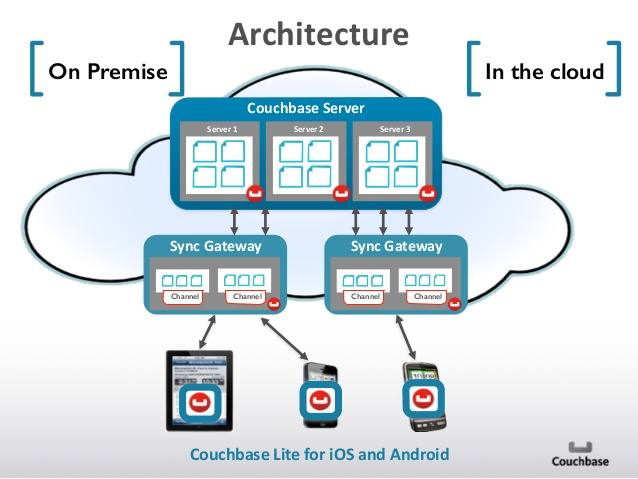
\includegraphics[width=\linewidth]{figures/Couchbase-Mobile-IOT-Database.jpg}
	 \caption{Couchbase Mobile Architecture}
  \label{fig: Couchbase Mobile Architecture}
\end{figure}			

		
\begin{description}
  \item[$\bullet$] {\bfseries Couchbase Lite:} Couchbase Lite is an lightweight embedded full featured JSON  document based and schemaless database on the device. It has APIs for Android,iOS and Rest along with integration support in popular cross-platform tools such as Phonegap and Xamarin. It includes features like peer-to-peer replication along with authorization by connecting with other mobile device running Couchbase Lite as its local storage and sync data with them after determining the document is replicated for that user.
 
    \item[$\bullet$] {\bfseries Couchbase Sync Gateway:} This component handles a two-way change synchronization between JSON store in Couchbase Server and Couchbase Lite.It  provides feature like routing required data to users avoid frequent network API calls, plug-in authentication, change validation and access control. 

  \item[$\bullet$] {\bfseries Couchbase Server:}	The NoSQL database that resides in the backend with elastic scalability and consistent high performance.
  
\end{description}


\subsection{Realm}

		Realm is a open source library launched in 2014 which can be integrated with the mobile application to store and query data. Realm introduced many features which made it appear as a replacement for SQLite.  

\begin{description}
  \item[$\bullet$] In this database , data is exposed as objects directly incorporating object relationships avoiding the need for ORM. At the same time, it remains extremely memory efficient. 
   \item[$\bullet$] It includes full ACID transactions default and an object schema is created directly driving from object definition.
   \item[$\bullet$] Unlike SQLite , Realm database are safe across threads making it highly concurrent when there is a burst of asynchronous task .  
\end{description}  


\section{Key - Value Database}

			Key-Value database is considered to be a simplest way storing data in the form of key-value pair and retrieving data based on key value. An advanced form of key-value store introduces the sorting of keys which enables an ordered processing of keys. Key-value database is also known as NoSQL databases. Key-Value store works differently when compared to relational database and it addresses several issues which relational database didn't address. Relational database 

\begin{description}
	\item[$\bullet$] Relational databases expects the schemas to be pre-defined which is poorly suited for agile development approaches as the schemas changes as the feature evolves.
	
\end{description}			
			
		
			
\subsection{Redis}
\subsection{Oracle NoSQL}
\subsection{MongoDB}

\section{Graph Database}

\subsection{Neo4j}
\subsection{Titan}







\section{In - Memory Database}

\subsection{Redis}
\subsection{Aerospike}

\section{Cloud Storage}

\subsection{Amazon S3}
\subsection{Amazon EBS}
\subsection{Google Cloud Storage}
\cleardoublepage
\chapter{Conclusion}\label{ch:conclusion}
In case you have questions, comments, suggestions or have found a bug, please do not hesitate to contact me. You can find my contact details below.
  \begin{center}
    Jesper Kjær Nielsen\\
    \href{mailto: jkn@es.aau.dk}{jkn@es.aau.dk}\\
    \href{http://kom.aau.dk/~jkn}{http://kom.aau.dk/\textasciitilde jkn}\\
    Fredrik Bajers Vej 7\\
    9220 Aalborg Ø
  \end{center}
\printbibliography[heading=bibintoc]
\label{bib:mybiblio}
\appendix
\chapter{Appendix A name}\label{ch:appAlabel}
Here is the first appendix
\end{document}